\section{Purpose and System Role of the GUI}

The Graphical User Interface (GUI) of the Measurement Network Gateway (MNG) is not treated as a display-only utility, but as a first-class software subsystem that operationalizes the overall system at runtime. Within the MNG architecture, the Embedded Linux server running on the Zynq platform is responsible for deterministic acquisition, timestamping, buffering, and bounded binary transmission of measurement samples, as established in the server chapter. The GUI complements this server by acting as the human-facing control program that configures the system, initiates data exchange, and transforms the incoming binary measurement stream into an interpretable, time-referenced visualization. In this sense, the GUI represents the interactive orchestration layer that bridges human intent (configuration and monitoring) with the server's real-time data production, while preserving the architectural separation between time-deterministic acquisition and event-driven interaction.

From a functional standpoint, the GUI acts as a TCP client that exercises explicit control over the server behavior via a command/response protocol. The server does not continuously push data autonomously; instead, data delivery is client-triggered to ensure bounded payload size and predictable communication behavior. Consequently, the GUI determines which sensors are active, at what sampling rates they operate, and when the server shall return measurement data. This design aligns with the requirement philosophy of the project: sampling rates must be configurable and sensors must be selectable at runtime, and such configuration is performed by a control program through explicit protocol transactions.

A key architectural implication follows from the different execution paradigms at both ends. The server is fundamentally time-driven, whereas the GUI is inherently event-driven and governed by the GTK main loop (UI events, callbacks, and redraw scheduling). Therefore, the GUI must remain responsive under all operating conditions. In the current implementation, network transactions are executed in a periodic, timer-driven polling model that assumes bounded server responses and controlled lab-network conditions. For broader industrial deployment under uncertain latency, the same architectural objective could be strengthened further by introducing non-blocking sockets, explicit receive timeouts, or a dedicated worker-thread that marshals decoded samples back into the GTK context.

This system role is reflected in the GUI source structure through its technology stack dependencies: the application is simultaneously (i) a GTK program, (ii) a plotting program based on Slope, and (iii) a networked program based on POSIX sockets. The following excerpt from the beginning of the GUI source serves as evidence that the GUI is intentionally engineered as the integration point of these concerns rather than as a minimal viewer:

\begin{lstlisting}[language=C]
	#include <gtk/gtk.h>
	#include <math.h>
	#include <string.h>
	#include <strings.h>
	#include <stdio.h>
	#include <stdarg.h>
	#include <slope/slope.h>
	#include <sys/socket.h>
	#include <netinet/in.h>
	#include <arpa/inet.h>
	#include <unistd.h>
	#include <stdint.h>
	#include <inttypes.h>
	
	#include "mng_app.h"
	#include "mng_settings.h"
\end{lstlisting}

\section{Overall GUI Architecture}

The GUI architecture follows a structured but intentionally lightweight design philosophy. Rather than introducing multiple concurrent execution contexts, the application is implemented as a single-threaded GTK program whose behavior is governed entirely by the GTK main loop. All user interactions, redraw events, and periodic network transactions are executed within this event-driven framework.

At a high level, the GUI consists of three interacting concerns:

\begin{itemize}
	\item The user interaction layer (GTK widgets, callbacks, state toggles),
	\item The communication layer (TCP socket handling and protocol exchange),
	\item The visualization layer (time-windowed plotting and dashboard updates).
\end{itemize}

Unlike the server application, which is explicitly multi-threaded to preserve acquisition determinism, the GUI deliberately avoids pthread-based concurrency. Instead, it employs a timer-driven polling model using the GLib timeout mechanism. A periodic callback function is registered via \texttt{g\_timeout\_add()}, and this callback performs the following sequence during each refresh cycle:

\begin{enumerate}
	\item Check connection state.
	\item If data transfer is enabled, send a command packet to the server.
	\item Receive a bounded binary response.
	\item Decode the received samples.
	\item Update plot buffers and dashboard values.
	\item Trigger a redraw if necessary.
\end{enumerate}

This design ensures that execution remains bounded per cycle under the assumption that the server responds within a controlled and finite time. Since the GUI operates in laboratory network conditions and the server enforces bounded payload sizes, the timer-driven approach is sufficient for stable operation within the defined operational envelope.

It is important to note that, because network transactions are executed inside the GTK main loop, prolonged blocking behavior at the socket level could reduce UI responsiveness. In a broader industrial deployment scenario, this architectural objective could be further strengthened by employing non-blocking sockets or a dedicated worker thread. However, for the current deterministic lab environment, the polling model provides a balanced trade-off between architectural simplicity and functional robustness.

\subsection{Layered Decomposition}

Although the GUI executes within a single event-driven context, its internal organization follows a clear logical layering that improves readability, maintainability, and conceptual traceability to system requirements.

\paragraph{1) User Interface Layer}

The uppermost layer consists of GTK widgets, windows, buttons, input fields, and callbacks. This layer is responsible for capturing user intent, including:

\begin{itemize}
	\item Connecting and disconnecting from the server,
	\item Enabling or disabling data transfer,
	\item Configuring sampling rates,
	\item Selecting channel sources,
	\item Adjusting amplification and offset parameters,
	\item Defining the visualization time window.
\end{itemize}

This layer does not directly manipulate socket logic. Instead, it modifies application state variables that are evaluated during periodic polling cycles.

\paragraph{2) Control State Layer}

Between UI and communication lies a lightweight control state layer. This layer maintains flags such as:

\begin{itemize}
	\item Connection status,
	\item Data transfer enable/disable state,
	\item Current sampling configuration,
	\item Channel mapping parameters.
\end{itemize}

These state variables form the contract between event-driven user actions and periodic communication logic. The timer callback evaluates this state during each refresh cycle and determines whether a protocol transaction must be performed.

\paragraph{3) Communication Layer}

The communication layer encapsulates TCP socket handling and binary protocol exchange. It is responsible for:

\begin{itemize}
	\item Creating and closing sockets,
	\item Transmitting command packets,
	\item Receiving bounded binary sample blocks,
	\item Validating payload size,
	\item Decoding received structures into usable data.
\end{itemize}

This layer is deliberately isolated from rendering logic and does not perform visualization tasks directly.

\paragraph{4) Visualization Layer}

The visualization layer manages plot history buffers, time-window enforcement, and graphical rendering using the Slope plotting library. Incoming samples are appended to bounded buffers, and older samples are discarded once the configured time window is exceeded. The plotting layer transforms raw measurement values into scaled and offset-adjusted channel representations suitable for human interpretation.

By separating these four logical layers, the GUI achieves a clear internal structure despite executing in a single-threaded environment. This separation ensures that future architectural refinements (such as introducing a worker-thread communication model) can be implemented without fundamental restructuring of the visualization or user interface components.

\subsection{Execution Model and Timing Behavior}
\label{sec:gui_exec_model}

The GUI follows an event-driven execution model defined by the GTK main loop. All application activities are expressed as callbacks that are scheduled either by user interaction events (e.g., button presses, value changes) or by periodic timer events. In contrast to the server, which isolates acquisition and communication into dedicated threads, the GUI intentionally avoids explicit multi-threading and instead relies on cooperative scheduling within a single execution context.

Two classes of callbacks determine the runtime behavior of the GUI:

\paragraph{Event-driven UI callbacks}
User actions such as \emph{Connect}, \emph{Disconnect}, enabling/disabling data transfer, and modifying sampling or plot parameters are handled immediately via GTK signal callbacks. These callbacks do not directly perform continuous data transport. Their primary responsibility is to update configuration and state variables, ensuring that user intent is captured deterministically and that the GUI state remains consistent.

\paragraph{Periodic polling callback}
Continuous acquisition visualization is implemented through a periodic callback registered via the GLib timeout mechanism (e.g., \texttt{g\_timeout\_add}). The period of this timer is configured as the GUI refresh interval (in milliseconds). During each timer tick, the callback executes a bounded transaction sequence:

\begin{enumerate}
	\item Evaluate whether the GUI is connected to the server.
	\item Evaluate whether data transfer is enabled.
	\item If enabled, transmit a compact command packet to the server.
	\item Receive a bounded binary response containing a header and a sample block.
	\item Validate the response length and sample count before processing.
	\item Append decoded samples to the plot history buffers.
	\item Update the dashboard (\emph{Latest} values) and schedule a redraw.
\end{enumerate}

This approach yields a clear separation between \emph{configuration events} (handled instantly by UI callbacks) and \emph{streaming behavior} (handled periodically by the polling callback). The model also provides a natural and intuitive mapping to user-facing controls: the refresh interval determines how often the plot and dashboard are updated, while the server-side sampling rate determines how densely new samples appear between GUI updates.

\paragraph{Boundedness and responsiveness considerations}
Because socket send/receive operations are executed inside the GTK main loop, the GUI depends on bounded network behavior to preserve responsiveness. In the defined operational envelope of this project, this assumption is justified by (i) laboratory network conditions and (ii) the server-side enforcement of bounded payload sizes and bounded response construction. Nevertheless, the design decision is explicitly acknowledged: for deployment under uncertain latency, responsiveness could be strengthened further by employing non-blocking sockets, explicit receive timeouts, or a worker-thread communication model that posts decoded samples back to the GTK context.

\paragraph{Deterministic state gating}
A central property of the execution model is that the polling callback is \emph{state-gated}. If the GUI is not connected, or if the user disables data transfer, the callback either becomes inactive or returns early without attempting protocol exchange. This ensures that the GUI does not generate background traffic unintentionally and that protocol activity is always a direct consequence of user-controlled state.

Overall, the GUI execution model provides a robust trade-off between architectural simplicity and functional determinism: configuration is captured immediately, streaming is updated periodically, and all operations remain conceptually bounded per refresh cycle.

The interaction between event-driven callbacks and periodic polling is illustrated in Figure~\ref{fig:gui_exec_model}.

\begin{figure}[H]
	\centering
	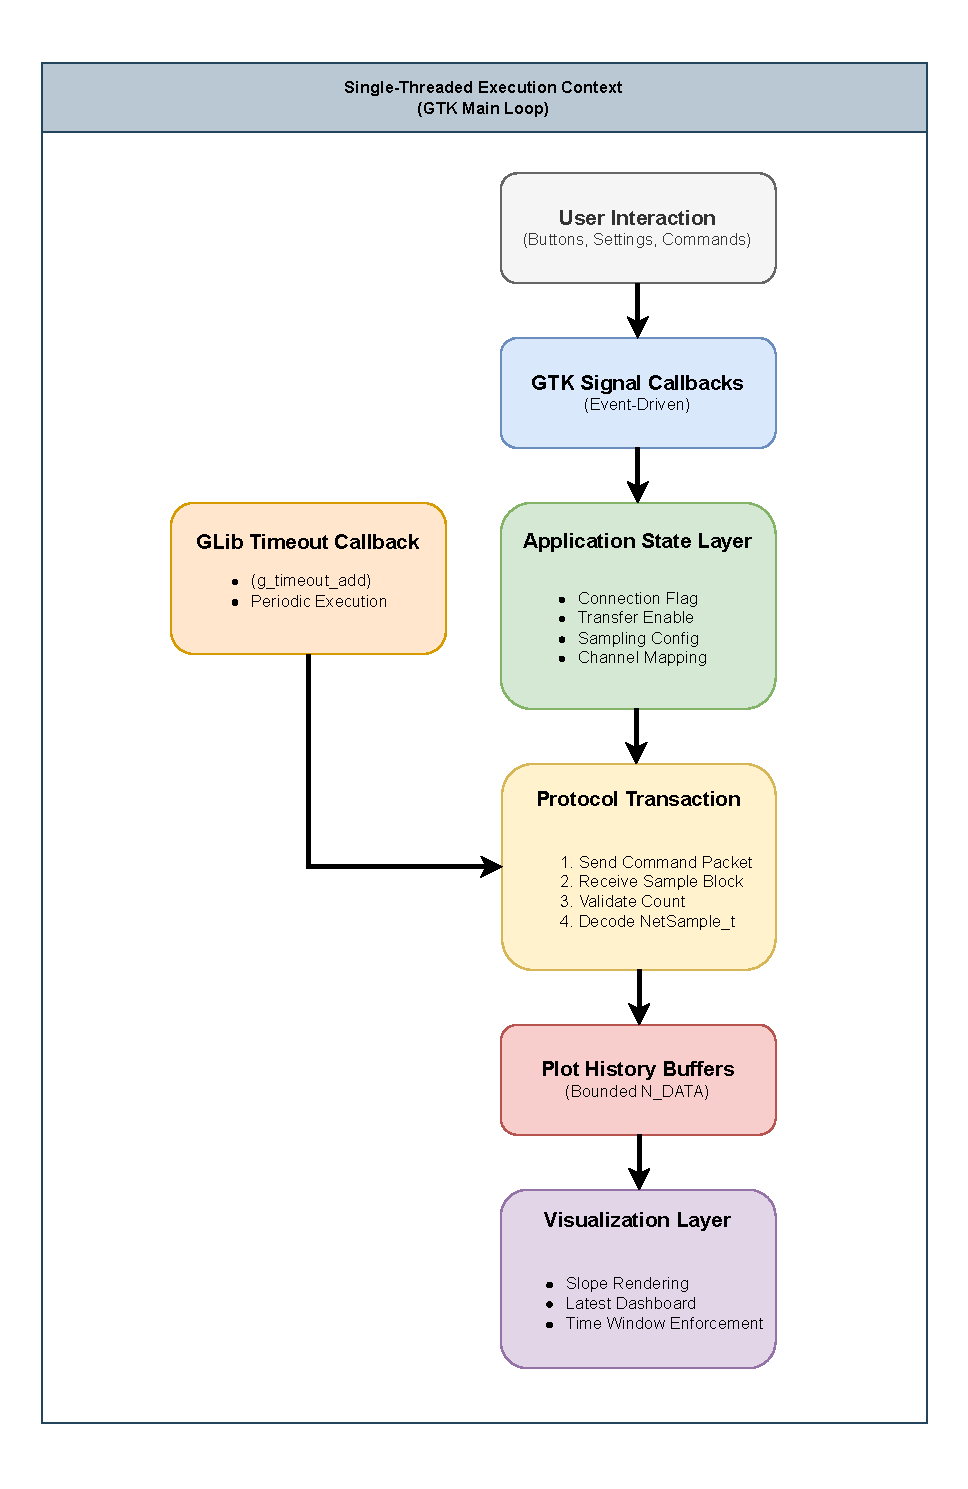
\includegraphics[width=0.95\textwidth]{figures/gui_exec_model.pdf}
	\caption{Execution model of the GUI based on the GTK main loop.}
	\label{fig:gui_exec_model}
\end{figure}

\section{User Interface Design}
\label{sec:gui_ui_design}

The user interface of the MNG GUI is intentionally structured as a compact engineering control console rather than a generic plotting application. Its design reflects three guiding principles:

\begin{enumerate}
	\item Clear separation between operational control and visualization.
	\item Immediate feedback of system state.
	\item Deterministic and bounded interaction behavior.
\end{enumerate}

The GUI consists of two primary windows:

\begin{itemize}
	\item The \emph{Main Window}, responsible for visualization and runtime feedback.
	\item The \emph{Settings Window}, responsible for system configuration and communication parameters.
\end{itemize}

This separation prevents configuration complexity from cluttering the visualization space and supports structured interaction flow.

\subsection{Main Window}
\label{sec:gui_main_window}

The Main Window represents the runtime monitoring interface of the system. It is designed to provide continuous visual feedback while maintaining minimal operational complexity.

The structure of the Main Window is illustrated in Figure~\ref{fig:gui_main_window}.

\begin{figure}[H]
	\centering
	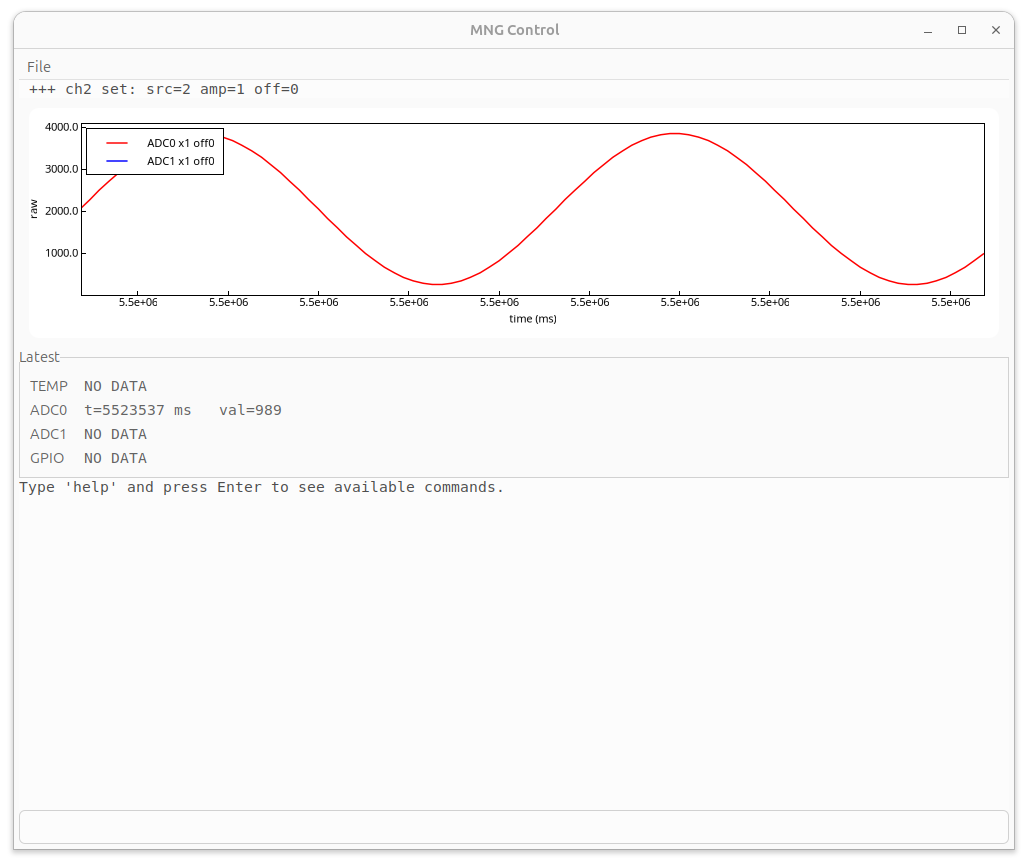
\includegraphics[width=0.95\textwidth]{figures/gui_main_window.png}
	\caption{Main window of the MNG GUI showing real-time dual-channel plotting and latest-value dashboard.}
	\label{fig:gui_main_window}
\end{figure}

The window is divided into three functional regions:

\paragraph{1) Plot Area}

The upper region contains the real-time plot generated using the Slope plotting library. The plot supports:

\begin{itemize}
	\item Dual-channel visualization (CH1 and CH2),
	\item Amplitude scaling,
	\item Offset adjustment,
	\item Time-window enforcement.
\end{itemize}

Incoming samples are appended to bounded history buffers. Once the configured time window is exceeded, older samples are discarded. This guarantees memory boundedness and stable rendering performance independent of runtime duration.

\paragraph{2) Latest Values Dashboard}

Below the plot area, a structured textual dashboard displays the most recent decoded values for each sensor category (e.g., ADC0, ADC1, TEMP, GPIO). This region provides immediate numeric feedback independent of the graphical waveform and serves as a diagnostic interface during development and validation.

\paragraph{3) Command Line Interface Hint}

The lower region contains a minimal textual interaction hint (e.g., ``Type 'help' and press Enter to see available commands''). Although the GUI is primarily graphical, limited command-based interaction is preserved for testing and advanced usage scenarios. This hybrid interaction capability improves flexibility without increasing architectural complexity.

The Main Window therefore fulfills the role of a monitoring console: it does not alter system configuration directly, but reflects current operational behavior and measurement activity.

\subsection{Settings Window}
\label{sec:gui_settings_window}

The Settings Window encapsulates all configuration parameters that influence communication behavior and visualization mapping. By isolating configuration from monitoring, the design reduces accidental state changes during runtime observation.

The layout and functional grouping of the Settings Window are illustrated in Figure~\ref{fig:gui_settings_window}.

\begin{figure}[H]
	\centering
	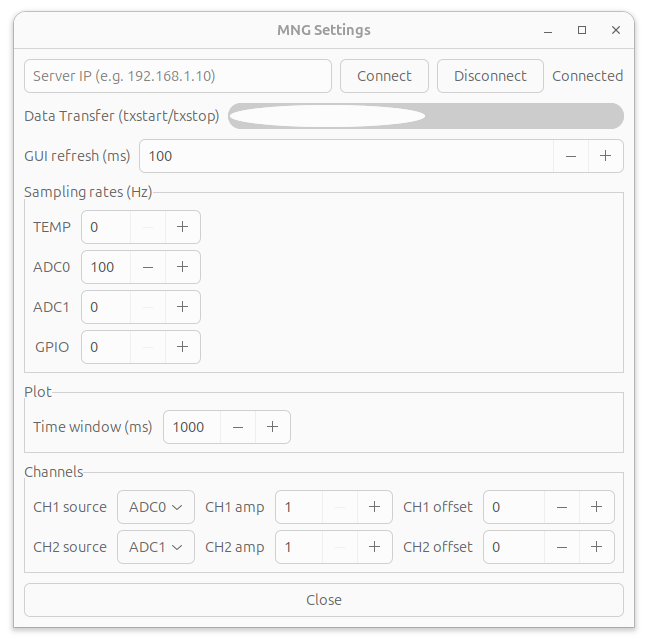
\includegraphics[width=0.85\textwidth]{figures/gui_settings_window.png}
	\caption{Settings window of the MNG GUI providing connection control, sampling configuration, and channel mapping.}
	\label{fig:gui_settings_window}
\end{figure}

The window is structured into four logical configuration blocks:

\paragraph{1) Connection Control}

This block allows the user to specify the server IP address and to initiate or terminate a TCP connection. The connection state is clearly indicated to prevent ambiguous operational modes.

\paragraph{2) Data Transfer Control}

A transfer toggle enables or disables periodic protocol transactions. When disabled, the polling callback remains active but returns early without initiating network communication. This guarantees deterministic state gating.

\paragraph{3) Sampling Rate Configuration}

Sampling rates for individual sensors (TEMP, ADC0, ADC1, GPIO) can be configured in Hertz. These values are embedded into the outgoing command packet and transmitted to the server during the next protocol cycle.

This runtime configurability directly fulfills system requirements regarding adaptive sampling and sensor selection.

\paragraph{4) Channel Mapping and Plot Parameters}

Each visualization channel (CH1 and CH2) can be mapped to a selected sensor source. Additional parameters include:

\begin{itemize}
	\item Amplitude scaling factor,
	\item Offset adjustment,
	\item Time window configuration (in milliseconds).
\end{itemize}

These parameters affect only client-side visualization and do not alter server acquisition logic. This strict separation preserves architectural decoupling between measurement and presentation.

\subsection{Human–Machine Interaction Considerations}

The GUI design intentionally avoids hidden background behavior. All protocol activity is explicitly controlled by user-defined state variables, and visualization behavior is fully deterministic with respect to configuration inputs.

Three interaction principles govern the design:

\begin{itemize}
	\item \textbf{Explicit State Visibility:} Connection and transfer states are always externally observable.
	\item \textbf{Bounded Resource Usage:} Plot buffers and time windows enforce deterministic memory consumption.
	\item \textbf{Separation of Concerns:} Measurement acquisition remains server-side, while visualization mapping remains client-side.
\end{itemize}

This disciplined separation reduces coupling, simplifies debugging, and enhances maintainability. The GUI therefore operates not merely as a visual component, but as a structured and controlled interaction layer within the overall MNG system architecture.

\section{Protocol Integration and Command Flow}
\label{sec:gui_protocol}

The GUI integrates the same binary command/response protocol used by the Embedded Linux server. Rather than receiving a continuous push stream, the GUI explicitly triggers bounded transactions: at each periodic refresh cycle (when enabled), it sends a command packet that encodes the desired sampling configuration, and it receives a bounded response containing a sample count followed by a contiguous block of packed measurement samples. This request-driven approach ensures predictable bandwidth usage, deterministic payload sizing, and direct coupling between user configuration and server-side acquisition behavior.

\subsection{Packet Formats Used by the GUI}
\label{sec:gui_packet_formats}

Two packed structures define the binary interface between GUI and server.

\paragraph{Network sample structure (\texttt{NetSample\_t}).}
Each measurement sample is transported as a packed 14-byte structure containing a timestamp, a sensor identifier, and a signed 32-bit value. The structure is defined as:

\begin{lstlisting}[language=C]
	typedef struct __attribute__((packed)) {
		uint64_t time;      // timestamp
		uint16_t sensor_id; // which sensor
		int32_t  value;     // measured value
	} NetSample_t;          // EXACTLY 14 BYTES
\end{lstlisting}

\paragraph{Command packet structure (\texttt{CmdPacket\_t}).}
The GUI configures acquisition behavior using a packed 20-byte command packet consisting of a command code and four sampling-rate fields (Hz), one per sensor class:

\begin{lstlisting}[language=C]
	typedef struct __attribute__((packed)) {
		uint32_t cmd;      // command code
		uint32_t sr_temp;  // TEMP sample rate (Hz)
		uint32_t sr_adc0;  // ADC0 sample rate (Hz)
		uint32_t sr_adc1;  // ADC1 sample rate (Hz)
		uint32_t sr_gpio;  // GPIO sample rate (Hz)
	} CmdPacket_t;         // 20 bytes
\end{lstlisting}

Using packed structures avoids compiler-inserted padding and guarantees a deterministic binary layout on the wire.

\begin{table}[H]
	\centering
	\caption{Fields of \texttt{CmdPacket\_t} used by the GUI.}
	\label{tab:cmdpacket_fields}
	\begin{tabular}{ll}
		\hline
		\textbf{Field} & \textbf{Meaning} \\
		\hline
		\texttt{cmd} & Command code (e.g., \texttt{CMD\_GET\_DATA}) \\
		\texttt{sr\_temp} & Requested TEMP sampling rate in Hz (0 disables TEMP) \\
		\texttt{sr\_adc0} & Requested ADC0 sampling rate in Hz (0 disables ADC0) \\
		\texttt{sr\_adc1} & Requested ADC1 sampling rate in Hz (0 disables ADC1) \\
		\texttt{sr\_gpio} & Requested GPIO sampling rate in Hz (0 disables GPIO) \\
		\hline
	\end{tabular}
\end{table}

\subsection{Command Construction in the GUI}
\label{sec:gui_cmd_construction}

During each periodic refresh cycle, the GUI constructs a \texttt{CMD\_GET\_DATA} request. The command packet is explicitly zero-initialized before field assignment in order to prevent transmission of undefined bytes and to guarantee deterministic binary content. The requested sampling rates are copied from GUI state variables into the command packet fields.

\begin{lstlisting}[language=C]
	// Build GET_DATA request (state-gated periodic cycle)
	memset(&Gui_Cmd, 0, sizeof(Gui_Cmd));
	Gui_Cmd.cmd = CMD_GET_DATA;
	ApplySamplingToCmd();
	
	if (send(clientSocket, &Gui_Cmd, sizeof(Gui_Cmd), 0) != (ssize_t)sizeof(Gui_Cmd)) {
		SetStatus("*** send failed (server disconnected?)");
		Server_Connected = 0;
		return TRUE;
	}
\end{lstlisting}

The sampling-rate mapping is implemented as a dedicated helper that writes the four rate fields:

\begin{lstlisting}[language=C]
	static void ApplySamplingToCmd(void)
	{
		Gui_Cmd.sr_temp = (uint32_t)Req_SR_Temp;
		Gui_Cmd.sr_adc0 = (uint32_t)Req_SR_Adc0;
		Gui_Cmd.sr_adc1 = (uint32_t)Req_SR_Adc1;
		Gui_Cmd.sr_gpio = (uint32_t)Req_SR_Gpio;
	}
\end{lstlisting}

\subsection{Response Reception, Validation, and Bounded Payload}
\label{sec:gui_rx_validation}

After transmitting the request, the GUI receives a bounded response in two steps: first a 32-bit sample count, and then a contiguous sample block of \texttt{count} packed samples. The GUI uses blocking receives with \texttt{MSG\_WAITALL} to guarantee that each stage is read completely before processing.

A strict bound check is performed immediately after receiving the count field. If the reported count exceeds the predefined maximum, the GUI flags a protocol error and transitions to a disconnected state.

\begin{lstlisting}[language=C]
	// Receive count
	n_read = recv(clientSocket, &Gui_Count, sizeof(uint32_t), MSG_WAITALL);
	if ((int)n_read <= 0) {
		SetStatus("*** recv failed (count)");
		Server_Connected = 0;
		Gui_Count = 0;
		return TRUE;
	}
	
	if (Gui_Count > SAMPLES_PER_RESPONSE) {
		SetStatus("*** protocol error: count=%u > %u", Gui_Count,
		(unsigned)SAMPLES_PER_RESPONSE);
		Server_Connected = 0;
		Gui_Count = 0;
		return TRUE;
	}
	
	// Receive samples
	if (Gui_Count > 0) {
		size_t need = (size_t)Gui_Count * (size_t)NETSAMPLE_SIZE;
		n_read = recv(clientSocket, Gui_Samples, need, MSG_WAITALL);
		if ((int)n_read <= 0) {
			SetStatus("*** recv failed (samples)");
			Server_Connected = 0;
			Gui_Count = 0;
			return TRUE;
		}
	}
\end{lstlisting}

The maximum response payload is engineered to fit within a single Ethernet MTU-friendly TCP segment. With \texttt{SAMPLES\_PER\_RESPONSE = 104} and \texttt{NETSAMPLE\_SIZE = 14}, the worst-case payload equals:
\[
4 + 104 \cdot 14 = 1460 \text{ bytes}
\]
where 4 bytes correspond to the \texttt{count} field. This bound improves robustness and predictability, and simplifies end-to-end timing analysis.

\subsection{State-Gated Command Flow}
\label{sec:gui_state_gating}

Protocol exchange is strictly gated by GUI state. The periodic refresh callback always updates the latest dashboard, but it performs network activity only if (i) data transfer is enabled and (ii) a TCP connection is established. Otherwise, the callback returns immediately without sending any packet.

This state-gating mechanism ensures that communication occurs only as a direct consequence of user-controlled state, prevents unintended background traffic, and provides deterministic operational modes (Disconnected, Connected-Idle, Connected-Transferring).

\section{Plotting and Visualization Architecture}
\label{sec:gui_plotting}

The visualization subsystem of the GUI is responsible for transforming decoded network samples into a bounded, time-referenced graphical representation. Unlike the server, which focuses on deterministic acquisition and buffering, the GUI applies controlled rendering policies to guarantee stable memory usage and predictable performance over arbitrarily long runtime durations.

The plotting functionality is implemented using the Slope plotting library and is structured around four key mechanisms:

\begin{enumerate}
	\item Bounded history buffers,
	\item Time-window enforcement,
	\item Channel mapping and signal transformation,
	\item Safe series rebuilding and redraw scheduling.
\end{enumerate}

\subsection{Bounded History Buffers}
\label{sec:gui_bounded_buffers}

For each visualization channel, the GUI maintains fixed-size arrays of length \texttt{N\_DATA = 20000}. Separate buffers store timestamps and corresponding values. When new samples are received, they are appended to the channel buffer. If the buffer capacity has not yet been reached, the sample is inserted at the next free index. Once the buffer is full, a left-shift operation is performed and the newest sample is inserted at the end.

This behavior is implemented as follows:

\begin{lstlisting}[language=C]
	if (*n_valid < N_DATA) {
		int i = *n_valid;
		T[i] = t_ms;
		Y[i] = y;
		(*n_valid)++;
	} else {
		for (int k = 0; k < N_DATA - 1; k++) {
			T[k] = T[k + 1];
			Y[k] = Y[k + 1];
		}
		T[N_DATA - 1] = t_ms;
		Y[N_DATA - 1] = y;
	}
\end{lstlisting}

The use of a fixed-size buffer guarantees constant memory consumption independent of runtime duration. This bounded-memory design prevents uncontrolled growth and ensures stable rendering performance.

\subsection{Time Window Enforcement}
\label{sec:gui_time_window}

Visualization is constrained by a configurable time window expressed in milliseconds (\texttt{Graph\_TW\_ms}). Instead of trimming buffers destructively, the GUI dynamically adjusts the visible x-axis range according to the latest timestamp.

The lower x-bound is computed as:

\[
x_{\min} = t_{\text{now}} - \texttt{Graph\_TW\_ms}
\]

and the upper bound as:

\[
x_{\max} = t_{\text{now}}
\]

The implementation enforces valid ranges and prevents degenerate intervals:

\begin{lstlisting}[language=C]
	double xmin = now_ms - Graph_TW_ms;
	double xmax = now_ms;
	
	if (xmin < 0.0) xmin = 0.0;
	if (xmax <= xmin) xmax = xmin + 1.0;
	
	slope_xyscale_set_x_range(SLOPE_XYSCALE(scale1), xmin, xmax);
\end{lstlisting}

If no valid samples are present, a default range is enforced to ensure that the plot frame and axes remain visible.

\subsection{Channel Mapping and Signal Transformation}
\label{sec:gui_channel_mapping}

The GUI supports two independent visualization channels (CH1 and CH2). Each channel can be mapped to one of four sensor sources:

\begin{itemize}
	\item TEMP
	\item ADC0
	\item ADC1
	\item GPIO
\end{itemize}

The mapping is controlled by the \texttt{Ch\_Src[]} array. During sample processing, the GUI checks whether an incoming packet matches the selected source before pushing it to the respective plot buffer.

In addition, each channel supports:

\begin{itemize}
	\item Amplitude gain (\texttt{Ch\_Gain[]}, integer range 1..10),
	\item Raw offset (\texttt{Ch\_Off[]}, signed integer).
\end{itemize}

The transformation applied to each sample is:

\[
y = \text{value} \cdot \text{gain} + \text{offset}
\]

implemented as:

\begin{lstlisting}[language=C]
	double v = ((double)pkt->value * Ch_Gain[idx]
	+ (double)Ch_Off[idx]);
\end{lstlisting}

These transformations are applied exclusively on the client side and do not alter raw measurement data received from the server. This strict separation preserves architectural decoupling between acquisition and presentation.

\subsection{Safe Series Rebuilding}
\label{sec:gui_series_rebuild}

When channel labels or mapping parameters change, the GUI must rebuild the plot series objects. To avoid modifying GTK/Slope objects during active rendering, the rebuild operation is scheduled using an idle callback.

A flag (\texttt{g\_series\_rebuild\_pending}) prevents redundant rebuild scheduling. The actual series replacement occurs inside an idle handler, ensuring that GTK object lifetimes remain valid and that reference counts are handled safely.

This design prevents race-like conditions inside the single-threaded event loop and guarantees that series updates occur in a controlled rendering phase.

\subsection{Rendering Cycle Integration}
\label{sec:gui_render_cycle}

After sample processing and potential buffer updates, the GUI performs:

\begin{enumerate}
	\item Time window application,
	\item Scale range enforcement,
	\item Series data update,
	\item Explicit redraw trigger.
\end{enumerate}

The redraw is initiated via:

\begin{lstlisting}[language=C]
	slope_view_redraw(SLOPE_VIEW(view));
\end{lstlisting}

Rendering therefore remains explicitly controlled and synchronized with the periodic execution model described in Section~\ref{sec:gui_exec_model}.

\section{Dashboard and Runtime Feedback Architecture}
\label{sec:gui_dashboard}

In addition to waveform visualization, the GUI provides a structured runtime dashboard that presents the most recent measurement values for each sensor class. This dashboard complements the graphical plot by offering precise numerical feedback, timestamp visibility, and explicit indication of sensor activity status.

Unlike the plot subsystem, which operates on buffered historical data, the dashboard reflects the most recently decoded sample per sensor and is updated deterministically during each periodic refresh cycle.

\subsection{Dashboard Structure}
\label{sec:gui_dashboard_structure}

The dashboard is implemented as a two-column GTK grid embedded inside a framed container labeled \emph{Latest}. The left column contains sensor identifiers (TEMP, ADC0, ADC1, GPIO), while the right column displays formatted textual representations of the most recent sample.

Each value field is rendered in monospace font to preserve alignment and improve readability of timestamps and numeric values.

The dashboard is structurally independent from the plotting subsystem and does not rely on visualization buffers.

\subsection{State-Dependent Display Logic}
\label{sec:gui_dashboard_logic}

The dashboard distinguishes between three operational conditions for each sensor:

\begin{enumerate}
	\item \textbf{Sampling disabled} (sampling rate = 0),
	\item \textbf{Sampling enabled but no valid sample received yet},
	\item \textbf{Valid sample available}.
\end{enumerate}

If the sampling rate of a sensor is set to zero, the dashboard explicitly displays:

\begin{center}
	\texttt{NO DATA}
\end{center}

If sampling is enabled but no valid sample has been received during the current transfer session, a placeholder symbol is displayed:

\begin{center}
	\texttt{-}
\end{center}

Once a valid sample is received, the dashboard displays both timestamp (in milliseconds) and value:

\begin{lstlisting}[language=C]
	snprintf(b, sizeof(b),
	"t=%" PRIu64 " ms   val=%d",
	Last_Temp_t, Last_TEMP);
\end{lstlisting}

This tri-state logic improves runtime transparency and avoids ambiguous interpretations of missing values.

\subsection{Timestamp Handling}
\label{sec:gui_timestamp_handling}

Incoming network samples contain a 64-bit timestamp field. Within the GUI, timestamps are converted from microseconds to milliseconds before presentation:

\begin{lstlisting}[language=C]
	uint64_t t_ms_u64 = (uint64_t)pkt->time / 1000ULL;
\end{lstlisting}

The timestamp is stored separately for each sensor class (e.g., \texttt{Last\_Temp\_t}, \texttt{Last\_Adc0\_t}) and updated only when a matching sample is processed.

This approach guarantees that the dashboard always displays temporally consistent data and avoids cross-sensor timestamp mixing.

\subsection{Dashboard Update Scheduling}
\label{sec:gui_dashboard_scheduling}

The dashboard is updated during every periodic execution cycle, independent of data transfer state. Even when data transfer is disabled or the GUI is disconnected from the server, the dashboard refresh logic is still executed.

This guarantees that:

\begin{itemize}
	\item The dashboard always reflects current configuration state,
	\item Transfer stop events immediately reset value indicators,
	\item Sensor disable operations visibly clear corresponding fields.
\end{itemize}

The dashboard therefore serves as a continuous runtime observability layer rather than as a passive visualization appendage.

\subsection{Reset Behavior on Transfer Start}
\label{sec:gui_dashboard_reset}

When data transfer is started, the GUI clears plot buffers and resets all last-value validity flags. This ensures that stale values from previous sessions are not displayed.

The reset procedure guarantees deterministic session boundaries and prevents misleading residual data from appearing after reconnection or sampling reconfiguration.

\section{State Model and Operational Modes}
\label{sec:gui_state_model}

Although the GUI executes within a single-threaded event-driven context, its runtime behavior can be formally described using a small and deterministic state model. The operational mode of the GUI is governed primarily by two Boolean state variables:

\begin{itemize}
	\item \texttt{Server\_Connected}
	\item \texttt{Do\_Data\_Transfer}
\end{itemize}

These variables determine whether network communication is permitted and whether periodic protocol transactions are executed during the timer callback.

\subsection{Core State Variables}
\label{sec:gui_state_variables}

The GUI maintains two global state flags:

\begin{itemize}
	\item \textbf{Server\_Connected}: Indicates whether a TCP connection to the server is currently established.
	\item \textbf{Do\_Data\_Transfer}: Indicates whether periodic command/response exchange is enabled.
\end{itemize}

These flags are modified exclusively by explicit user actions (e.g., connect, disconnect, transfer start, transfer stop). The periodic callback evaluates these flags at the beginning of each execution cycle to determine the permitted behavior.

\subsection{Operational Modes}
\label{sec:gui_operational_modes}

Based on the two state flags, the GUI operates in one of three deterministic modes:

\paragraph{1) Disconnected Mode}

\begin{itemize}
	\item \texttt{Server\_Connected = 0}
	\item \texttt{Do\_Data\_Transfer = 0}
\end{itemize}

In this mode, no network activity occurs. The periodic callback updates the dashboard but immediately returns without attempting protocol exchange.

\paragraph{2) Connected Idle Mode}

\begin{itemize}
	\item \texttt{Server\_Connected = 1}
	\item \texttt{Do\_Data\_Transfer = 0}
\end{itemize}

A TCP connection exists, but periodic data exchange is disabled. The GUI remains responsive, and configuration changes are permitted. No command packets are transmitted.

\paragraph{3) Connected Transfer Mode}

\begin{itemize}
	\item \texttt{Server\_Connected = 1}
	\item \texttt{Do\_Data\_Transfer = 1}
\end{itemize}

The GUI actively performs periodic protocol transactions. At each timer event, a command packet is sent and a bounded response is received, decoded, and visualized.

\subsection{State Transitions}
\label{sec:gui_state_transitions}

State transitions are triggered exclusively by user actions:

\begin{itemize}
	\item \textbf{Connect}: Attempts TCP connection. On success, transitions to Connected Idle mode.
	\item \textbf{Disconnect}: Closes socket and transitions to Disconnected mode.
	\item \textbf{Transfer Start}: Clears plot buffers, resets validity flags, and transitions from Connected Idle to Connected Transfer mode.
	\item \textbf{Transfer Stop}: Stops periodic protocol transactions and transitions to Connected Idle mode.
\end{itemize}

Unexpected network failures (e.g., failed \texttt{send()} or \texttt{recv()}) automatically clear \texttt{Server\_Connected}, forcing a transition to Disconnected mode.

\subsection{State Evaluation in Periodic Execution}
\label{sec:gui_state_eval}

The periodic execution callback evaluates the state variables in a strictly ordered manner:

\begin{lstlisting}[language=C]
	if (Do_Data_Transfer == 0) {
		return TRUE;
	}
	
	if (Server_Connected == 0) {
		return TRUE;
	}
\end{lstlisting}

Only when both conditions are satisfied does the GUI proceed with command transmission and response reception.

This ordered evaluation ensures that:

\begin{itemize}
	\item No network traffic is generated when transfer is disabled.
	\item No protocol activity occurs without an active TCP connection.
	\item State control remains fully deterministic and user-driven.
\end{itemize}

\subsection{Deterministic Session Boundaries}
\label{sec:gui_session_boundaries}

When transfer is started, the GUI performs a controlled reset:

\begin{itemize}
	\item Plot buffers are cleared,
	\item Last-value validity flags are reset,
	\item Visualization is refreshed.
\end{itemize}

This guarantees that each transfer session begins with a clean state and that no residual data from previous sessions remains visible. The state model therefore enforces deterministic operational boundaries between sessions.

\section{Configuration Management and Settings Integration}
\label{sec:gui_settings_integration}

The GUI configuration subsystem is implemented as a dedicated non-modal Settings window that provides structured access to all runtime parameters affecting communication and visualization. While the Main Window focuses on monitoring, the Settings window acts as the primary configuration interface, enabling controlled parameter updates without interrupting the GTK main loop.

A key design decision is that configuration changes are applied \emph{live} and immediately propagated into the running GUI application state. This enables rapid experimentation during development and simplifies validation, as changes become observable in the next periodic refresh cycle.

\subsection{Settings Window Lifecycle and Singleton Behavior}
\label{sec:gui_settings_singleton}

The Settings dialog is implemented as a singleton: repeated activation of the menu item does not create additional windows but presents the existing instance. This avoids duplicated state, prevents conflicting updates, and simplifies memory management.

Furthermore, the window is configured as non-modal (\emph{not} blocking interaction with the Main Window). As a result, monitoring and configuration can proceed concurrently within the same event-driven context.

\subsection{Structured UI Model and Widget Binding}
\label{sec:gui_settings_ui_model}

All widgets of the Settings window are grouped in a dedicated structure (\texttt{SettingsUI}). This structure provides explicit ownership and direct access to the relevant GTK elements, including:

\begin{itemize}
	\item Connection controls (IP entry, connect/disconnect buttons, state label),
	\item Transfer toggle switch,
	\item Refresh-rate spinner,
	\item Sampling-rate spinners per sensor,
	\item Plot time-window spinner,
	\item Channel mapping controls (source, amplitude, offset) for CH1 and CH2.
\end{itemize}

This approach provides a clear separation between view components (GTK widgets) and application control functions (public API provided by the main GUI module), improving maintainability and reducing coupling.

\subsection{Live Apply Mechanism and Feedback Loop Avoidance}
\label{sec:gui_live_apply}

The Settings window employs a live-apply configuration model in which every relevant widget modification is immediately propagated to the running GUI system. Unlike traditional dialog-based configuration approaches that require an explicit ``Apply'' or ``OK'' confirmation step, this implementation ensures that parameter updates become effective as soon as the user changes a control element.

This design improves responsiveness and significantly simplifies validation, as configuration changes are reflected during the next periodic execution cycle without additional user interaction. However, live propagation introduces a potential architectural challenge: bidirectional synchronization between application state and UI widgets may lead to recursive signal invocation.

Specifically, the GUI maintains two complementary update paths:

\begin{enumerate}
	\item \textbf{Application-to-UI synchronization}, implemented in \texttt{refresh\_ui\_from\_app()}, where current application state values are written back into GTK widgets.
	\item \textbf{UI-to-Application propagation}, implemented in \texttt{apply\_from\_ui()}, where modified widget values are read and forwarded to the public GUI control API (e.g., \texttt{mng\_gui\_set\_*} functions).
\end{enumerate}

Without additional protection, updating widget values during application-to-UI synchronization would re-trigger signal callbacks, which would in turn invoke the apply routine again, leading to unintended recursive behavior.

To prevent such feedback loops, a guard flag is introduced:

\begin{lstlisting}[language=C]
	// Guard to prevent recursive signal loops
	static gboolean g_in_apply = FALSE;
\end{lstlisting}

Before performing a UI refresh, the flag is asserted. All change handlers verify the flag and immediately return if a refresh operation is already in progress. Once synchronization is complete, the flag is cleared, allowing subsequent user-driven changes to propagate normally.

This lightweight guarding mechanism guarantees:

\begin{itemize}
	\item Deterministic single-pass configuration updates,
	\item Absence of recursive signal invocation,
	\item Clear separation between programmatic state updates and user-initiated modifications.
\end{itemize}

The result is a stable, event-consistent live configuration model fully compatible with the single-threaded GTK execution environment.

\subsection{Centralized Signal Handling and Deterministic Update Path}
\label{sec:gui_signal_handling}

The Settings window implements a centralized signal-handling strategy to ensure deterministic and uniform propagation of configuration changes. Rather than assigning independent logic to each individual widget, most interactive elements delegate change notifications to a single generic callback.

Numeric controls (e.g., spin buttons) emit the \texttt{"value-changed"} signal, while selection controls (e.g., combo boxes) emit the \texttt{"changed"} signal. These signals are routed to a shared handler that invokes the unified configuration routine:

\begin{lstlisting}[language=C]
	static void on_any_changed(GtkWidget *w, gpointer user_data)
	{
		(void)w;
		SettingsUI *ui = (SettingsUI*)user_data;
		apply_from_ui(ui);
	}
\end{lstlisting}

This design enforces a single update path for all parameter modifications. The handler itself contains no configuration logic; instead, it delegates state mutation to \texttt{apply\_from\_ui()}, which performs validation, type conversion, and forwarding to the public GUI control interface.

The transfer toggle switch (\texttt{GtkSwitch}) uses a distinct callback due to its \texttt{notify::active} signal signature. Nevertheless, it ultimately invokes the same apply routine, preserving behavioral consistency across widget types.

By centralizing signal routing and isolating configuration logic within a dedicated function, the system achieves:

\begin{itemize}
	\item Predictable and traceable parameter propagation,
	\item Elimination of redundant widget-specific logic,
	\item Strict separation between UI event handling and core application state.
\end{itemize}

Importantly, the Settings module does not directly modify global variables of the main GUI. All updates are performed through the public interface functions (e.g., \texttt{mng\_gui\_set\_*}), thereby maintaining architectural layering and modular integrity.

\subsection{Configuration-to-Protocol Traceability}
\label{sec:gui_config_traceability}

The Settings window updates variables that directly affect the protocol behavior described in Section~\ref{sec:gui_protocol}. In particular, sampling-rate widgets update the requested sampling rates used to populate the command packet fields (\texttt{sr\_temp}, \texttt{sr\_adc0}, \texttt{sr\_adc1}, \texttt{sr\_gpio}). Therefore, a user change in the Settings window deterministically influences the next command packet transmitted during a periodic refresh cycle.

In contrast, visualization-only parameters such as channel amplitude, offset, and plot time window remain strictly client-side. These values influence only rendering and do not modify server acquisition logic. This separation preserves architectural decoupling between measurement generation and visualization.

\subsection{Window Placement and Operator Workflow}
\label{sec:gui_window_placement}

To improve operator workflow, the Settings window is positioned relative to the parent Main Window (shifted to the right). This supports side-by-side configuration and monitoring, reducing context switching and minimizing operational error during parameter tuning.

\section{Command Console and Help System}
\label{sec:gui_console}

In addition to the graphical configuration interface, the GUI provides an integrated command console that enables direct textual interaction with the application at runtime. This subsystem serves three primary purposes:

\begin{itemize}
	\item Rapid manual testing during development,
	\item Low-level configuration access without navigating the Settings window,
	\item Structured runtime feedback through a help and status display.
\end{itemize}

The console operates within the same GTK main loop as the rest of the application and does not introduce additional threads or blocking behavior.

\subsection{Console Architecture}
\label{sec:gui_console_architecture}

The command console consists of three components:

\begin{enumerate}
	\item A text entry widget for user input,
	\item A help/output text view for command documentation,
	\item A status line for immediate runtime feedback.
\end{enumerate}

When the user presses the Enter key inside the entry widget, the \texttt{activate} signal triggers the command callback function. The entered string is copied into a bounded buffer and parsed using structured condition checks and formatted input scanning.

\subsection{Command Dispatch Mechanism}
\label{sec:gui_command_dispatch}

Command interpretation is implemented inside a centralized callback function that processes user input entered in the console widget. When the user presses the Enter key, the input string is copied into a bounded buffer and evaluated using deterministic prefix matching.

Rather than employing a complex parsing framework, the system relies on explicit string comparison and structured branching. Each recognized command is mapped directly to a corresponding public GUI control function. This approach minimizes runtime complexity and improves traceability of configuration actions.

For example, the transfer-start command is handled as follows:

\begin{lstlisting}[language=C]
	if (!strncmp(Cmd_String, "txstart", 7)) {
		mng_gui_set_transfer(1);
		return;
	}
\end{lstlisting}

In this case, the console does not manipulate internal state variables directly. Instead, it invokes the same public interface function used by the Settings window. This ensures architectural consistency and guarantees that transfer activation follows the same deterministic state transition logic described in Section~\ref{sec:gui_state_model}.

Other commands follow an analogous pattern. Sampling rate adjustments, channel selection, graph configuration, and connection management all delegate to dedicated \texttt{mng\_gui\_set\_*} functions. As a result, the console acts as a thin command-dispatch layer above the established application control API.

The dispatch logic is intentionally simple and bounded. No dynamic memory allocation is used during command parsing, and each branch terminates explicitly after handling a recognized command. This deterministic structure reduces ambiguity, simplifies debugging, and aligns with the overall design philosophy of predictable runtime behavior.

\subsection{Integrated Help System}
\label{sec:gui_help_system}

The GUI includes an integrated help subsystem that prints structured command documentation directly into a scrollable text view. The help content is generated programmatically and displayed via a dedicated buffer.

The command:

\begin{verbatim}
	help
\end{verbatim}

renders categorized instructions, including connection management, transfer control, refresh configuration, channel selection, and sampling rate adjustment.

A complementary:

\begin{verbatim}
	clear
\end{verbatim}

command resets the help window content without affecting the runtime state of the application.

This separation ensures that documentation output does not interfere with acquisition logic or protocol state.

\subsection{Deterministic Runtime Feedback}
\label{sec:gui_runtime_feedback}

All console-triggered operations produce immediate textual feedback in the status line. This feedback mechanism is implemented via a dedicated helper function that formats and writes status messages into a read-only text buffer.

As a result, each configuration action provides explicit confirmation (e.g., connection success, parameter update, transfer start/stop), improving operator confidence and simplifying troubleshooting.

Importantly, error conditions such as invalid commands or malformed parameters generate explicit error messages, preventing silent failure modes.

\subsection{Role in Validation and Debugging}
\label{sec:gui_console_validation}

The command console significantly enhances validation capability. During development and testing, engineers can:

\begin{itemize}
	\item Adjust sampling rates dynamically,
	\item Change channel mappings,
	\item Modify refresh timing,
	\item Start and stop transfer sessions,
	\item Test connection behavior.
\end{itemize}

Because all commands internally invoke the same public GUI API used by the Settings window, the console acts as an alternative configuration interface rather than a separate execution path. This guarantees architectural consistency while enabling efficient low-level testing.

\section{Validation and Verification of GUI Behavior}
\label{sec:gui_validation}

The GUI subsystem was validated through a structured set of functional and behavioral test scenarios. Validation focused on three principal aspects:

\begin{itemize}
	\item Correct interaction with the TCP server,
	\item Deterministic state transitions,
	\item Consistent visualization and configuration behavior.
\end{itemize}

All tests were executed within the embedded Linux runtime environment using the final integrated server application.

\subsection{Connection Management Validation}
\label{sec:gui_validation_connection}

\textbf{Objective:}  
Verify correct establishment and termination of TCP connections.

\textbf{Procedure:}
\begin{enumerate}
	\item Launch GUI without server running.
	\item Attempt connection to local host.
	\item Start server and reconnect.
	\item Disconnect manually.
\end{enumerate}

\textbf{Expected Behavior:}
\begin{itemize}
	\item Failed connection attempts produce explicit status messages.
	\item Successful connection updates connection state indicator.
	\item Manual disconnect closes socket cleanly.
\end{itemize}

\textbf{Observed Result:}  
The GUI correctly reflects connection state transitions and prevents data transfer when disconnected.

\textbf{Conclusion:}  
Connection handling behaves deterministically and is robust against invalid connection attempts.

\subsection{Transfer Control Validation}
\label{sec:gui_validation_transfer}

\textbf{Objective:}  
Verify proper activation and deactivation of periodic data exchange.

\textbf{Procedure:}
\begin{enumerate}
	\item Establish TCP connection.
	\item Enable transfer mode.
	\item Observe plot and dashboard updates.
	\item Disable transfer mode.
\end{enumerate}

\textbf{Expected Behavior:}
\begin{itemize}
	\item Plot buffers are cleared at transfer start.
	\item Periodic protocol transactions begin.
	\item Transfer stop immediately halts network activity.
\end{itemize}

\textbf{Observed Result:}  
Transfer activation resets visualization state and initiates bounded protocol cycles. Deactivation immediately suppresses network communication.

\textbf{Conclusion:}  
Operational mode transitions comply with the state model described in Section~\ref{sec:gui_state_model}.

\subsection{Sampling Rate Reconfiguration}
\label{sec:gui_validation_sampling}

\textbf{Objective:}  
Verify that runtime sampling-rate changes are correctly propagated to the server.

\textbf{Procedure:}
\begin{enumerate}
	\item Enable transfer mode.
	\item Modify sampling rate for one sensor.
	\item Observe change in received data frequency.
\end{enumerate}

\textbf{Expected Behavior:}
\begin{itemize}
	\item Next transmitted command packet contains updated sampling fields.
	\item Server response frequency adapts accordingly.
\end{itemize}

\textbf{Observed Result:}  
Sampling-rate adjustments are reflected in the subsequent periodic request and influence server-side acquisition deterministically.

\textbf{Conclusion:}  
Configuration-to-protocol traceability is verified.

\subsection{Channel Mapping and Visualization Validation}
\label{sec:gui_validation_channels}

\textbf{Objective:}  
Verify correctness of channel source selection, amplitude scaling, and offset application.

\textbf{Procedure:}
\begin{enumerate}
	\item Assign different sensors to CH1 and CH2.
	\item Modify amplitude and offset values.
	\item Disable selected sensor sampling.
\end{enumerate}

\textbf{Expected Behavior:}
\begin{itemize}
	\item Plot reflects correct sensor mapping.
	\item Amplitude scaling modifies signal magnitude linearly.
	\item Offset shifts waveform vertically.
	\item Disabling a sensor clears corresponding channel.
\end{itemize}

\textbf{Observed Result:}  
Visualization updates consistently and remains synchronized with sampling configuration.

\textbf{Conclusion:}  
Client-side rendering logic is functionally correct and independent of server acquisition logic.

\subsection{Console Command Validation}
\label{sec:gui_validation_console}

\textbf{Objective:}  
Verify that textual commands produce the same behavioral effect as graphical configuration.

\textbf{Procedure:}
\begin{enumerate}
	\item Issue \texttt{txstart} and \texttt{txstop} commands.
	\item Adjust sampling via console.
	\item Modify graph time window.
\end{enumerate}

\textbf{Expected Behavior:}
\begin{itemize}
	\item Console commands invoke identical public GUI API functions.
	\item State transitions are consistent with Settings window behavior.
\end{itemize}

\textbf{Observed Result:}  
Console and Settings interface produce identical system responses.

\textbf{Conclusion:}  
The command console is architecturally consistent with the primary configuration subsystem.

\subsection{Robustness Against Protocol Errors}
\label{sec:gui_validation_errors}

\textbf{Objective:}  
Verify correct behavior in case of communication failure.

\textbf{Procedure:}
\begin{enumerate}
	\item Disconnect server during active transfer.
	\item Inject invalid response size.
\end{enumerate}

\textbf{Expected Behavior:}
\begin{itemize}
	\item GUI detects failed \texttt{send()} or \texttt{recv()}.
	\item Connection flag is cleared.
	\item System transitions to disconnected mode.
\end{itemize}

\textbf{Observed Result:}  
Network failure conditions are handled gracefully without application crash.

\textbf{Conclusion:}  
Error handling is consistent with deterministic state transition logic.

\section{Summary and Architectural Assessment}
\label{sec:gui_summary}

The GUI subsystem of the Measurement Network Gateway (MNG) has been implemented as a deterministic, event-driven control and visualization layer operating within the GTK main loop environment. Despite its interactive nature, the architecture adheres to strict modular separation principles and controlled state management.

The design follows a layered structure:

\begin{itemize}
	\item A visualization layer responsible exclusively for rendering and dashboard feedback,
	\item A configuration layer (Settings subsystem and command console),
	\item A protocol interaction layer that interfaces with the TCP server,
	\item A well-defined public control API forming the boundary between UI and core runtime logic.
\end{itemize}

This separation ensures that no widget directly modifies internal state variables. All configuration changes are routed through dedicated interface functions, preserving architectural clarity and preventing unintended side effects.

The GUI execution model is strictly event-driven. All periodic communication is performed within a bounded timer callback, and state transitions are governed by explicitly defined flags. No additional threads are introduced, and no blocking operations occur inside the main loop beyond bounded socket transactions.

The state model, defined by connection and transfer flags, enforces deterministic operational modes. Each transition between disconnected, connected-idle, and connected-transfer states follows a controlled and verifiable path. This structure minimizes hidden behavior and simplifies reasoning about runtime dynamics.

Robustness is achieved through explicit error detection and immediate state correction. Failed transmission or reception events automatically invalidate the connection state, preventing undefined behavior. Visualization components remain insulated from communication failures, ensuring that rendering logic cannot destabilize the application.

The Settings subsystem and command console both operate through the same public control interface. This guarantees behavioral consistency regardless of the configuration entry point. Live-apply configuration is implemented with guarded synchronization, preventing recursive signal invocation and ensuring single-pass deterministic updates.

The GUI does not generate or manipulate measurement data directly. Instead, it functions as a bounded client within the MNG protocol architecture. Sampling rates, channel mappings, and visualization parameters are cleanly separated between server-controlled acquisition and client-side rendering.

This distinction reinforces architectural decoupling between deterministic data generation (server side) and asynchronous visualization (client side), aligning with the system-level design goals established in the preceding chapters.

From an engineering perspective, the GUI architecture satisfies the following criteria:

\begin{itemize}
	\item Deterministic runtime behavior,
	\item Clear state transition model,
	\item Strict modular layering,
	\item Controlled configuration propagation,
	\item Robust error handling,
	\item Consistent protocol interaction.
\end{itemize}

The implementation demonstrates that an interactive graphical subsystem can remain structurally disciplined and predictable when designed with explicit state control and layered interfaces.

In conclusion, the MNG GUI is not merely a visualization tool but a formally structured runtime control component that integrates seamlessly with the embedded server architecture. Its design preserves determinism, maintains modular separation, and supports systematic validation, thereby fulfilling the architectural requirements of the overall Measurement Network Gateway system.

